\documentclass[letter,11pt]{article}

\usepackage[spanish,es-nodecimaldot]{babel}
\usepackage[utf8]{inputenc}

\usepackage{lmodern}
\usepackage[T1]{fontenc}
\usepackage{textcomp}

\usepackage{framed}
\usepackage[svgnames]{xcolor}
\colorlet{shadecolor}{Gainsboro!50}

\usepackage[labelfont=bf]{caption}
\usepackage{graphicx}
\usepackage{pstricks}

\usepackage{anysize}
\marginsize{3cm}{2cm}{2cm}{3cm}

\usepackage{siunitx}
\usepackage{amsmath}
\usepackage{array}
\usepackage{csquotes}
\usepackage{steinmetz}
\usepackage{stmaryrd}
\usepackage{multirow}

\usepackage{fancyhdr}
\usepackage{lastpage}
\pagestyle{fancy}
\fancyhf{}
\fancyhead[LE,RO]{Laboratorio de Circuitos Eléctricos III}
\fancyfoot[CO,CE]{\thepage\ de \pageref{LastPage}}

\special{papersize=215.9mm,279.4mm}

\usepackage[
    pdfauthor={Carlos Eduardo Caballero Burgoa},%
    pdftitle={Laboratorio de Circuitos Eléctricos III},%
    pdfsubject={Medida del factor de potencia trifásico},%
    colorlinks,%
    citecolor=black,%
    filecolor=black,%
    linkcolor=black,%
    urlcolor=black,
    breaklinks]{hyperref}
\usepackage{breakurl}

\renewcommand{\arraystretch}{1.2}

\begin{document}

\begin{titlepage}
    \begin{center}
        {\Large UNIVERSIDAD MAYOR DE SAN SIMÓN}\\
        \vspace*{0.15cm}
        {\large FACULTAD DE CIENCIAS Y TECNOLOGÍA}\\
        \vspace*{0.10cm}
        DEPARTAMENTO DE ELÉCTRICA-ELECTRÓNICA\\
        \vspace*{3.0cm}
        {\Large \textbf{LABORATORIO DE CIRCUITOS ELÉCTRICOS III}}\\
        \vspace*{0.3cm}
        {\Large \textbf{INFORME No. 8}}\\
        \vspace*{3.5cm}
        {\Large \textbf{CORRECCIÓN DEL FACTOR DE POTENCIA TRIFÁSICO\\
        EN CARGAS EQUILIBRADAS}}\\
    \end{center}

    \vspace*{5.3cm}
    \leftskip=7.95cm
    \noindent
    \textbf{Estudiante:}\\
    Caballero Burgoa, Carlos Eduardo.\\
    \newline
    \textbf{Carrera:}\\
    Ing. Electromecánica.\\
    \newline
    \textbf{Docente:}\\
    Ing. Marco Antonio Vallejo Camacho.\\
    \newline
    \textbf{Grupo:} 2F (Martes).\\
\textbf{Fecha de entrega:} 26 de Noviembre del 2024.\\
\end{titlepage}

\section{Cálculos teóricos}
Considerando un circuito trifásico con carga en estrella equilibrado, se hallan
los factores de potencia, las corrientes de linea y las potencias activa,
reactiva y aparente.

\subsection{Carga $RL$}
\begin{figure}[!h]
\centering
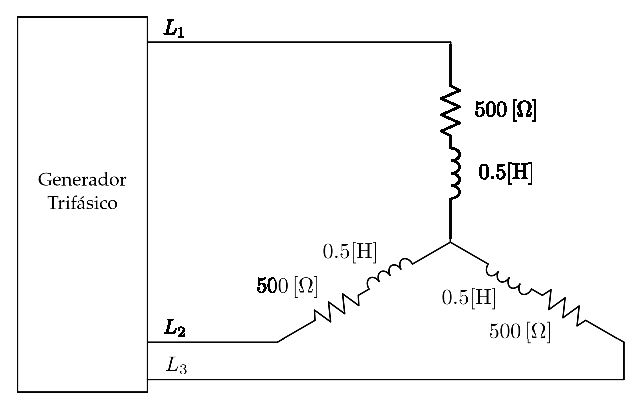
\includegraphics[scale=0.9]{figura1.eps}
\caption{Circuito trifásico equilibrado con carga $RL$.}
\label{circuito1}
\end{figure}

Considerando un circuito trifásico con carga $RL$ estrella equilibrado
(\textbf{Figura~\ref{circuito1}}).

Se calcula la frecuencia angular ($\omega$):
\begin{equation*}
    \begin{split}
        \omega&=2\pi f\\
              &=2\pi(50)\\
              &=100\pi\,[\text{rad}/\text{s}]\\
    \end{split}
\end{equation*}

Se halla la impedancia en el dominio de frecuencia:
\begin{equation*}
    \begin{split}
        Z &= R+j\omega L\\
          &= 500+j\,(100\pi)\,(0.5)\\
          &= 500+j50\pi\,[\Omega]\\
    \end{split}
\end{equation*}

Y su representación fasorial:
\begin{equation*}
    \begin{split}
        |Z| &= \sqrt{500^2+(50\pi)^2}\\
            &= 524.09\\
        \theta &= \arctan\left(\frac{50\pi}{500}\right)\\
               &= 17.44^{\circ}\\
        Z &= 524.09\phase{17.44^{\circ}}\,[\Omega]\\
    \end{split}
\end{equation*}

Por tanto, el factor de potencia es:
\begin{equation*}
    \begin{split}
        \text{fp} &= \cos(17.44^{\circ})\\
                  &= 0.9540\,\text{(atrasado)}\\
    \end{split}
\end{equation*}

A partir del voltaje de linea, se calcula el voltaje de fase:
\begin{equation*}
    \begin{split}
        U_F &= \frac{U_L}{\sqrt{3}}\\
            &= \frac{380}{\sqrt{3}}\\
            &= 219.39[\text{V}]\\
    \end{split}
\end{equation*}

Y a partir del voltaje de fase, se halla la corriente de linea:
\begin{equation*}
    \begin{split}
        I_L &= \frac{U_F}{|Z|}\\
            &= \frac{219.39}{\sqrt{(500)^2+(50\pi)^2}}\\
            &= 0.4186[\text{A}]\\
    \end{split}
\end{equation*}

Por tanto, las potencias activa, reactiva y aparente son:
\begin{equation*}
    \begin{split}
        P_T &= \sqrt{3}\,U_L\,I_L\,\cos(\phi)\\
            &= \sqrt{3}\,(380)\,(0.4186)\,\cos(17.44^{\circ})\\
            &= 262.86[\text{W}]\\
        Q_T &= \sqrt{3}\,U_L\,I_L\,\sen(\phi)\\
            &= \sqrt{3}\,(380)\,(0.4186)\,\sen(17.44^{\circ})\\
            &= 82.579[\text{VAR}]\\
        S_T &= \sqrt{(262.86)^2+(82.579)^2}\\
            &= 275.52[\text{VA}]\\
    \end{split}
\end{equation*}

\subsection{Carga $RL$ con capacitor en serie}
\begin{figure}[!h]
\centering
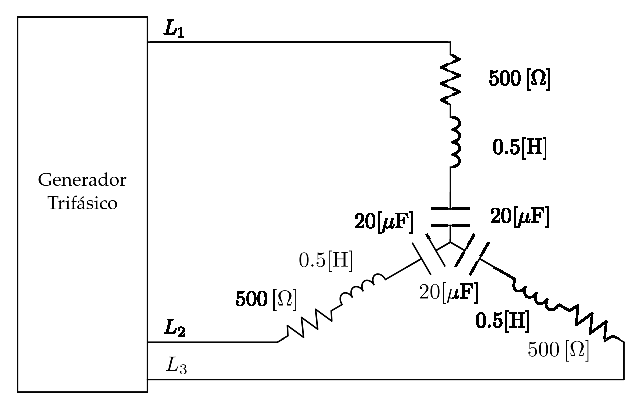
\includegraphics[scale=0.9]{figura2.eps}
\caption{Circuito trifásico equilibrado con \\carga $RL$ y capacitor en serie.}
\label{circuito2}
\end{figure}

Considerando un circuito trifásico con carga $RLC$ estrella equilibrado
(\textbf{Figura~\ref{circuito2}}).

Se halla la impedancia en el dominio de frecuencia:
\begin{equation*}
    \begin{split}
        Z &= R+j\omega L+\frac{1}{j\omega C}\\
          &= 500+j\,(100\pi)\,(0.5)+\frac{1}{j\,(100\pi)\,(\num{20e-6})}\\
          &= 500-j2.0753\,[\Omega]\\
    \end{split}
\end{equation*}

Y su representación fasorial:
\begin{equation*}
    \begin{split}
        |Z| &= \sqrt{500^2+(-2.0753)^2}\\
            &= 500.00\\
        \theta &= \arctan\left(\frac{-2.0753}{500}\right)\\
               &= -0.24^{\circ}\\
        Z &= 500.00\phase{-0.24^{\circ}}\,[\Omega]\\
    \end{split}
\end{equation*}

Por tanto, el factor de potencia es:
\begin{equation*}
    \begin{split}
        \text{fp} &= \cos(-0.24^{\circ})\\
                  &= 1.0000\,\text{(adelantado)}\\
    \end{split}
\end{equation*}

A partir del voltaje de linea, se calcula el voltaje de fase:
\begin{equation*}
    \begin{split}
        U_F &= \frac{U_L}{\sqrt{3}}\\
            &= \frac{380}{\sqrt{3}}\\
            &= 219.39[\text{V}]\\
    \end{split}
\end{equation*}

Y a partir del voltaje de fase, se halla la corriente de linea:
\begin{equation*}
    \begin{split}
        I_L &= \frac{U_F}{|Z|}\\
            &= \frac{219.39}{\sqrt{(500)^2+(-2.0753)^2}}\\
            &= 0.4388[\text{A}]\\
    \end{split}
\end{equation*}

Por tanto, las potencias activa, reactiva y aparente son:
\begin{equation*}
    \begin{split}
        P_T &= \sqrt{3}\,U_L\,I_L\,\cos(\phi)\\
            &= \sqrt{3}\,(380)\,(0.4388)\,\cos(-0.24^{\circ})\\
            &= 288.80[\text{W}]\\
        Q_T &= \sqrt{3}\,U_L\,I_L\,\sen(\phi)\\
            &= \sqrt{3}\,(380)\,(0.4388)\,\sen(-0.24^{\circ})\\
            &= -1.1987[\text{VAR}]\\
        S_T &= \sqrt{(288.80)^2+(-1.1987)^2}\\
            &= 288.80[\text{VA}]\\
    \end{split}
\end{equation*}

\subsection{Carga $RL$ con capacitor en paralelo}
\begin{figure}[!h]
\centering
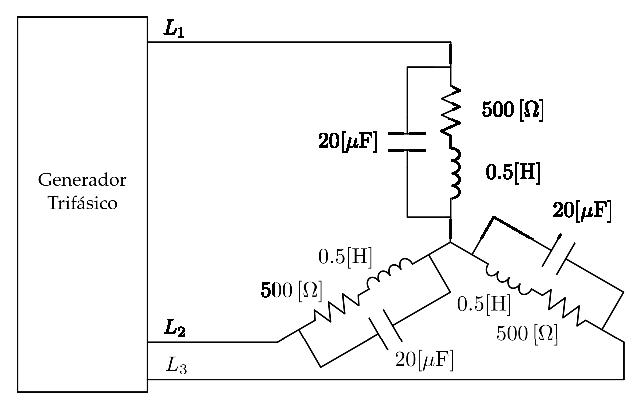
\includegraphics[scale=0.9]{figura3.eps}
\caption{Circuito trifásico equilibrado con \\
carga $RL$ y capacitor en paralelo.}
\label{circuito3}
\end{figure}

Considerando un circuito trifásico con carga $RLC$ estrella equilibrado
(\textbf{Figura~\ref{circuito3}}).

Se halla la impedancia en el dominio de frecuencia:
\begin{equation*}
    \begin{split}
        Z &= (R+j\omega L)||(\frac{1}{j\omega C})\\
          &= \frac{(500+j50\pi)(-j\frac{500}{\pi})}
             {(500+j50\pi)+(-j\frac{500}{\pi})}\\
          &= 50.660-j158.945\,[\Omega]\\
    \end{split}
\end{equation*}

Y su representación fasorial:
\begin{equation*}
    \begin{split}
        |Z| &= \sqrt{(50.660)^2+(-158.945)^2}\\
            &= 166.82\\
        \theta &= \arctan\left(\frac{-158.945}{50.660}\right)\\
               &= -72.32^{\circ}\\
        Z &= 166.82\phase{-72.32^{\circ}}\,[\Omega]\\
    \end{split}
\end{equation*}

Por tanto, el factor de potencia es:
\begin{equation*}
    \begin{split}
        \text{fp} &= \cos(-72.32^{\circ})\\
                  &= 0.3037\,\text{(adelantado)}\\
    \end{split}
\end{equation*}

A partir del voltaje de linea, se calcula el voltaje de fase:
\begin{equation*}
    \begin{split}
        U_F &= \frac{U_L}{\sqrt{3}}\\
            &= \frac{380}{\sqrt{3}}\\
            &= 219.39[\text{V}]\\
    \end{split}
\end{equation*}

Y a partir del voltaje de fase, se halla la corriente de linea:
\begin{equation*}
    \begin{split}
        I_L &= \frac{U_F}{|Z|}\\
            &= \frac{219.39}{\sqrt{(50.660)^2+(-158.945)^2}}\\
            &= 1.3151[\text{A}]\\
    \end{split}
\end{equation*}

Por tanto, las potencias activa, reactiva y aparente son:
\begin{equation*}
    \begin{split}
        P_T &= \sqrt{3}\,U_L\,I_L\,\cos(\phi)\\
            &= \sqrt{3}\,(380)\,(1.3151)\,\cos(-72.32^{\circ})\\
            &= 262.86[\text{W}]\\
        Q_T &= \sqrt{3}\,U_L\,I_L\,\sen(\phi)\\
            &= \sqrt{3}\,(380)\,(1.3151)\,\sen(-72.32^{\circ})\\
            &= -824.71[\text{VAR}]\\
        S_T &= \sqrt{(262.86)^2+(-824.71)^2}\\
            &= 865.59[\text{VA}]\\
    \end{split}
\end{equation*}

\subsection{Resumen de resultados}
En la siguiente tabla se resumen los valores obtenidos teóricamente:

\begin{center}
    \begin{tabular}{|c||c|c|c|c|c|}
    \hline
    & $I_F[\text{A}]$ &
    $P_T[\text{W}]$ &
    $Q_T[\text{VAR}]$ &
    $S_T[\text{VA}]$ &
    \text{fp}
    \tabularnewline \hline \hline
    $RL$ &
    $0.4186$ &
    $262.86$ &
    $82.58$ &
    $275.52$ &
    $0.9540\,\text{(atrasado)}$
    \tabularnewline \hline
    $RL$ + C en serie &
    $0.4388$ &
    $288.80$ &
    $-1.20$ &
    $288.80$ &
    $1.0000\,\text{(adelantado)}$
    \tabularnewline \hline
    $RL$ + C en paralelo &
    $1.3151$ &
    $262.86$ &
    $-824.71$ &
    $865.59$ &
    $0.3037\,\text{(adelantado)}$
    \tabularnewline \hline
    \end{tabular}
\end{center}

\section{Simulación}
Se utilizó el software \emph{Electronic Workbench v5.12.} para simular
los circuitos, la carga $RL$ puede verse en la
\textbf{Figura~\ref{simulacion1}}, la carga $RL$ con capacitor en serie puede
verse en la \textbf{Figura~\ref{simulacion2}} y la carga $RL$ con capacitor en
paralelo puede verse en la \textbf{Figura~\ref{simulacion3}}.

\begin{figure}[!h]
\centering
\includegraphics[scale=0.98]{simulacion/practica8.1.eps}
\caption{Simulación de la carga $RL$.}
\label{simulacion1}
\end{figure}

\begin{figure}[!h]
\centering
\includegraphics[scale=0.98]{simulacion/practica8.2.eps}
\caption{Simulación de la carga $RL$ con capacitor en serie.}
\label{simulacion2}
\end{figure}

\begin{figure}[!h]
\centering
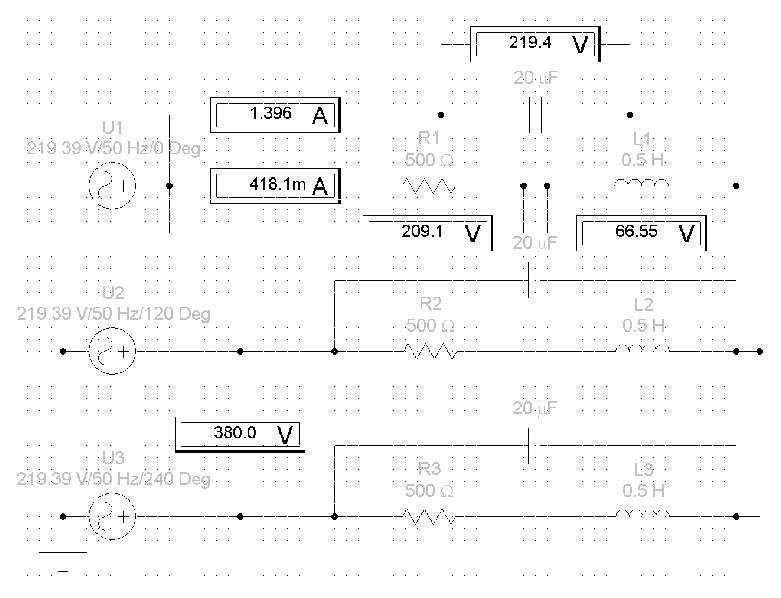
\includegraphics[scale=0.98]{simulacion/practica8.3.eps}
\caption{Simulación de la carga $RL$ con capacitor en paralelo.}
\label{simulacion3}
\end{figure}

\subsection{Resumen de resultados}
En la siguiente tabla se resumen los valores obtenidos de la simulación: 

\begin{center}
    \begin{tabular}{|c||c|c|c|c|c|}
    \hline
    & $I_F[\text{A}]$ &
    $P_T[\text{W}]$ &
    $Q_T[\text{VAR}]$ &
    $S_T[\text{VA}]$ &
    \text{fp}
    \tabularnewline \hline \hline
    $RL$ &
    $0.4183$ &
    $262.27$ &
    $83.51$ &
    $275.25$ &
    $0.9529$
    \tabularnewline \hline
    $RL$ + C en serie &
    $0.4389$ &
    $288.75$ &
    $1.16$ &
    $288.75$ &
    $1.0000$
    \tabularnewline \hline
    $RL$ + C en paralelo &
    $1.8141$ &
    $262.27$ &
    $-835.37$ &
    $875.58$ &
    $0.2995$
    \tabularnewline \hline
    \end{tabular}
\end{center}

\section{Tablas y mediciones}
Se presentan los resultados obtenidos en laboratorio por medio del método de los
dos vatímetros, el calculo de la potencia activa, reactiva, aparente y el factor
de potencia.

La potencia aparente se calcula con la siguiente formula:
\begin{equation*}
    S_T = \sqrt{P_T^2 + Q_T^2}
\end{equation*}

El factor de potencia se calcula con la siguiente formula:
\begin{equation*}
    \text{fp} = \frac{P_T}{S_T}
\end{equation*}

\begin{center}
    \begin{tabular}{|c||c|c|c|c|c|}
    \hline
    & $I_F[\text{A}]$ &
    $W_1 + W_2 = P_T[\text{W}]$ &
    $Q_1 + Q_2 = Q_T[\text{VAR}]$ &
    $S_T[\text{VA}]$ &
    \text{fp}
    \tabularnewline \hline \hline
    $RL$ &
    $0.40$ &
    $110 + 153 = 263$ &
    $112 - 31 = 81$ &
    $275.19$ &
    $0.9557$
    \tabularnewline \hline
    $RL$ + C en serie &
    $0.42$ &
    $143 + 143 = 286$ &
    $79 - 78 = 1$ &
    $286$ &
    $1.0000$
    \tabularnewline \hline
    $RL$ + C en paralelo &
    $1.40$ &
    $390 - 126 = 264$ &
    $-393 - 528 = -921$ &
    $958.09$ &
    $0.2755$
    \tabularnewline \hline
    \end{tabular}
\end{center}

\section{Cuestionario}

\begin{enumerate}

\item \textbf{¿Qué efectos produce en el circuito un mayor factor de potencia?
Justifique su respuesta con los datos obtenidos.}

Considerando que el factor de potencia se calcula con la siguiente formula:
\begin{equation*}
    \begin{split}
        \text{fp} &= \frac{P_T}{S_T}\\
        S_T &= \sqrt{P_T^2 + Q_T^2}\\
    \end{split}
\end{equation*}

El valor del factor de potencia se halla comprendido en el intervalo $[0,1]$,
para subir el factor de potencia debe aproximarse la potencia activa ($P_T$) a
la potencia aparente ($S_T$), es decir, reducir la potencia reactiva ($Q_T$).

En el caso de la medición de laboratorio el circuito $RC$ tiene los siguientes
valores:
\begin{equation*}
    \begin{split}
        P_T &= 263[\text{W}]\\
        Q_T &= 81[\text{VAR}]\\
        S_T &= 275.19[\text{VA}]\\
        \text{fp} &= \frac{263}{275.19}\\
                  &= 0.9557\\
    \end{split}
\end{equation*}

Con la conexión de un capacitor en serie los nuevos valores son:
\begin{equation*}
    \begin{split}
        P_T &= 286[\text{W}]\\
        Q_T &= 1[\text{VAR}]\\
        S_T &= 286[\text{VA}]\\
        \text{fp} &= \frac{286}{286}\\
                  &= 1.0000\\
    \end{split}
\end{equation*}

El factor de potencia $1$ indica que toda la energía consumida por los
componentes ha sido transformada en trabajo.

\item \textbf{¿Qué efectos produce en el circuito un menor factor de potencia?
Justifique su respuesta con los datos obtenidos.}

En el caso de la medición de laboratorio el circuito $RC$ tiene los siguientes
valores:
\begin{equation*}
    \begin{split}
        P_T &= 263[\text{W}]\\
        Q_T &= 81[\text{VAR}]\\
        S_T &= 275.19[\text{VA}]\\
        \text{fp} &= \frac{263}{275.19}\\
                  &= 0.9557\\
    \end{split}
\end{equation*}

Con la conexión de un capacitor en paralelo los nuevos valores son:
\begin{equation*}
    \begin{split}
        P_T &= 264[\text{W}]\\
        Q_T &= -921[\text{VAR}]\\
        S_T &= 958.09[\text{VA}]\\
        \text{fp} &= \frac{264}{958.09}\\
                  &= 0.2755\\
    \end{split}
\end{equation*}

La reducción del factor de potencia indica menor eficiencia en el consumo de la
energía.

\item \textbf{¿Por qué razón es conveniente conectar capacitancias en paralelo
en vez de conectar en serie cuando se corrige el factor de potencia? Justifique
su respuesta}

Un \textbf{capacitor en serie} compensa la reactancia inductiva. En otras
palabras, un capacitor en serie es una reactancia negativa (capacitiva) en serie
con la reactancia positiva (inductiva) del circuito con el efecto de compensar
parte o  la totalidad de ella. Por lo tanto, el efecto principal del capacitor
en serie es minimizar, o incluso suprimir, la caída de voltaje causada por la
reactancia inductiva en el circuito.

Un capacitor serie proporciona un aumento de voltaje que aumenta automática e
instantáneamente a medida que aumenta la carga. Además, un capacitor serie
produce más aumento de voltaje neto que un capacitor en paralelo a factores de
potencia más bajos, lo que crea más caída de voltaje. Sin embargo, un capacitor
serie mejora el factor de potencia del sistema mucho menos que un capacitor en
paralelo y tiene poco efecto sobre la corriente de la fuente.

Un \textbf{capacitor en paralelo} suministran el tipo de potencia reactiva o
corriente para contrarrestar el componente fuera de fase de la corriente
requerida por una carga inductiva.

En cierto sentido, los capacitores en paralelo modifican la característica de
una carga inductiva al generar una corriente principal que contrarresta parte o
la totalidad del componente retrasado de la corriente de carga inductiva en el
punto de instalación.

Mediante la aplicación de un capacitor en paralelo, la magnitud de la fuente de
corriente se puede reducir, el factor de potencia se puede mejorar y, en
consecuencia, la caída de voltaje entre el extremo de envío y la carga también
se reduce \cite{Merla}.

\item \textbf{Calcular cual debería ser el valor de la capacitancia en paralelo
a conectarse por fase para obtener un factor de potencia igual a 1.}

Calculando la impedancia equivalente:
\begin{equation*}
    \begin{split}
        Z_{\text{eq}}
            &= \dfrac{(500+j50\pi)\left(-j\dfrac{1}{100\pi{C}}\right)}
               {500+j50\pi-j\dfrac{1}{100\pi{C}}}\\
            &= \dfrac{-j\dfrac{500}{100\pi{C}}+\dfrac{50\pi}{100\pi{C}}}
               {500+j\left(50\pi-\dfrac{1}{100\pi{C}}\right)}\\
            &= \dfrac{\dfrac{1}{2C}-j\dfrac{5}{\pi{C}}}
               {500+j\left(\dfrac{5000\pi^2{C}-1}{100\pi{C}}\right)}\\
            &= \dfrac{\dfrac{1}{2C}-j\dfrac{5}{\pi{C}}}
               {500+j\left(\dfrac{5000\pi^2{C}-1}{100\pi{C}}\right)}
               \dfrac{500-j\left(\dfrac{5000\pi^2{C}-1}{100\pi{C}}\right)}
               {500-j\left(\dfrac{5000\pi^2{C}-1}{100\pi{C}}\right)}\\
            &= \dfrac
               {\left(\dfrac{1}{2C}-j\dfrac{5}{\pi{C}}\right)
               \left(500-j\dfrac{5000\pi^2{C}-1}{100\pi{C}}\right)}
               {500^2+\left(\dfrac{5000\pi^2{C}-1}{100\pi{C}}\right)^2}\\
    \end{split}
\end{equation*}
\begin{equation*}
    \begin{split}
        Z_{\text{eq}}
            &= \dfrac
               {\dfrac{250}{C}-j\dfrac{5000\pi^2{C}-1}{200\pi{C^2}}
               -j\dfrac{2500}{\pi{C}}-\dfrac{5000\pi^2{C}-1}{20\pi^2{C^2}}}
               {500^2+\left(\dfrac{5000\pi^2{C}-1}{100\pi{C}}\right)^2}\\
            &= \dfrac{\dfrac{250}{C}-\dfrac{5000\pi^2{C}-1}{20\pi^2{C^2}}}
               {500^2+\left(\dfrac{5000\pi^2{C}-1}{100\pi{C}}\right)^2}-
               j\dfrac{\dfrac{5000\pi^2{C}-1}{200\pi{C^2}}+\dfrac{2500}{\pi{C}}}
               {500^2+\left(\dfrac{5000\pi^2{C}-1}{100\pi{C}}\right)^2}\\
    \end{split}
\end{equation*}

Considerando que el factor de potencia es $1$ cuando la parte imaginaria de la
impedancia equivalente es $0$, entonces:
\begin{equation*}
    \dfrac{\dfrac{5000\pi^2{C}-1}{200\pi{C^2}}+\dfrac{2500}{\pi{C}}}
    {500^2+\left(\dfrac{5000\pi^2{C}-1}{100\pi{C}}\right)^2}=0
\end{equation*}
\begin{equation*}
    \frac{5000\pi^2{C}-1}{200\pi{C^2}}=-\frac{2500}{\pi{C}}
\end{equation*}
\begin{equation*}
    5000\pi^2{C}-1=-500000{C}
\end{equation*}
\begin{equation*}
    5000\pi^2{C}+500000{C}=1
\end{equation*}
\begin{equation*}
    \begin{split}
        C &= \frac{1}{5000\pi^2+500000}\\
          &= \num{1.82e-6}[\text{F}] = 1.82[\mu\text{F}]\\
    \end{split}
\end{equation*}

\end{enumerate}

\section{Conclusiones y Recomendaciones}
Se midieron los valores en un circuito con carga estrella equilibrada, y se
midieron los factores de potencia agregando un capacitor en serie y paralelo.

Se puede observar también como la precisión del vatímetro varia ligeramente los
cálculos de potencia y factor de potencia.

Es recomendable realizar la simulación del circuito antes de conectar
componentes adicionales para la corrección del factor de potencia, ya que puede
rebasar la potencia que es capaz de disipar el componente.

\begin{thebibliography}{99}

\bibitem{Merla} Merla, Alfonso (2021, Junio).\\
La diferencia en como los capacitores serie y en derivación regulan el voltaje
y los flujos de potencia reactiva.\\
Extraído el 24 de Noviembre del 2024, de:\\
https://cursostesla.com/la-diferencia-en-como-los-capacitores-serie-y-en-derivacion-regulan-el-voltaje-y-los-flujos-de-potencia-reactiva/

\end{thebibliography}
\end{document}

